\documentclass{article}
\usepackage{tikz}

\begin{document}

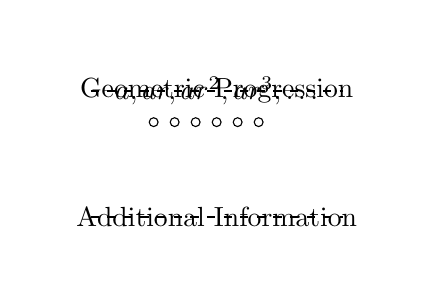
\begin{tikzpicture}[scale=0.8]
    % Whiteboard background
    \fill[white] (0,0) rectangle (6,4);

    % Geometric Progression Formula
    \node at (3,3) {
        $a, ar, ar^2, ar^3, \ldots$
    };

    % Related Paths - Geometric Progression Dots
    \foreach \i in {0,1,...,5} {
        \draw (2+\i/3, 2.5) circle (2pt);
    }

    % Unrelated Paths - Additional Shapes
    \draw[thick, dashed] (1,1) -- (5,1); % Horizontal line
    \draw[thick, dashed] (1,3) -- (5,3); % Horizontal line

    \node at (3,1) {Additional Information};
    \node at (3,3) {Geometric Progression};

\end{tikzpicture}

\end{document}